\chapter{State of the Art}
\chaptermark{State of the Art}
\label{chapter:soa}
\minitoc

%%%%%%%%%%%%%%%%%%%%%%%%%%%%%%%%%%%%%%%%%%%%%%%%%%%%%%%%%%%%%%%%%%%%%%%%%%%%%%%%%%%%%%%%%%%%%%%
\section{Introduction}
This chapter provides an overview of related work to contextualize the primary objectives of the thesis. Firstly, in Section~\ref{section:ift}, Information Flow Tracking (IFT) is introduced, detailing the different types and their respective purposes. We discuss the various levels of monitoring, from program behaviour to the detection of hardware trojans.
Then, in Section~\ref{section:physicalAttacks}, we provide an overview of the different existing physical attacks, focusing on Fault Injection Attacks (FIAs).
Finally, in Section~\ref{section:countermeasuresAgainstFIA}, we present existing countermeasures against FIAs.

% %%%%%%%%%%%%%%%%%%%%%%%%%%%%%%%%%%%%%%%%%%%%%%%%%%%%%%%%%%%%%%%%%%%%%%%%%%%%%%%%%%%%%%%%%%%%%%%
\section{Information Flow Tracking}
\label{section:ift}
The concept of \textit{Information Flow Tracking} has been introduced by the work of Bell and LaPadula~\cite{BLP-76-military} and by Denning~\cite{D-76-commacm} in 1976.
This section introduces Information Flow Tracking mechanisms, explains how they work, and presents the various types of IFT with their different functional levels.

%%%%%%%%%%%%%%%%%%%%%%%%%%%%%%%%
\subsection{How hardware DIFT works}
DIFT is a technique used in computer security to monitor the flow of information through a system. It aims to prevent security breaches such as data leaks, unauthorised data manipulation, and execution of untrusted code. In DIFT, each data is associated with a tag that indicates its security level.
For example, a tag might indicate whether a data is 'trusted' or 'untrusted'. When a data is input into the system, it is initially tagged based on its source.

As data moves through the system, these tags are tracked to ensure compliance with security policies and to ensure that sensitive information does not get exposed or manipulated improperly. For instance, if an operation involves both trusted and untrusted data, the result might be tagged as untrusted to ensure security.

An example of such security policy can be represented in Table~\ref{table:security_policies}. In this example, if the data comes from the network or if it's manipulated by a user, in the case of a \verb|scanf()| function in C language for example, the data cannot be trusted, while if the data comes from a secure channel or is manipulated by the system itself, the data can be trusted.

\begin{table}[ht]
    \centering
    \caption{Security policies for different data inputs}
    \label{table:security_policies}
    \begin{tabular}{@{}rcc@{}}
        \toprule
        \textbf{Data Input} & \textbf{Security Policy} & \textbf{Tag}     \\ \midrule
        User Input          & User-provided            & Untrusted        \\ \hline
        Network             & External source          & Untrusted        \\ \hline
        Internal            & System-provided          & Trusted          \\
        \bottomrule
    \end{tabular}
\end{table}

Figure~\ref{fig:dift_init} illustrates the three main steps of how DIFT works. Firstly, three data, $D_1$, $D_2$, and $D_3$, with their associated tags in two different colours, are initialised on the left side of the figure.
In the second step, when the data are fetched by the core for computation, the associated tags are propagated inside the core and confronted with the propagation policy depending on the operations performed on the data.
Finally, in the last step, on the right side of the figure, there are two data outputs derived from the three initial data. Data $D_4$ results from the combination of data $D_2$ and $D_3$, while data $D_5$ is derived only from data $D_1$. Since data $D_1$ has not been modified, its tag remains the same. However, the tag associated to $D_4$ is the combination of tags from $D_2$ and $D_3$. Depending on the security policy, if $D_3$ was trusted and $D_2$ was not, the output tag will be \textit{untrusted} (i.e, as in the Figure~\ref{fig:dift_init}). Consequently, when the tags go through the final step of DIFT, they will be checked, and an exception may be raised, or the application may be stopped due to the combination of \textit{trusted} and \textit{untrusted} values.

\begin{figure}[ht]
    \centering
    \includegraphics[page=3]{c2_soa/img/schemaDIFT.pdf}
    \caption{Representation of the DIFT mechanism from initialisation to checking.}
    \label{fig:dift_init}
\end{figure}
    
%%%%%%%%%%%%%%%%%%%%%%%%%%%%%%%%
\subsection{Different types of IFT}
There are two distinct types of IFT approaches: static and dynamic, each with its own specific objectives.

\subsubsection{Static IFT}
Static Information Flow Tracking (SIFT) is a security technique used to analyse and control the flow of information within a program or system without executing it, by examining the source code or compiled binary~\cite{HAK-21-acmcsur}. This method is particularly useful for identifying theoretical vulnerabilities, ensuring compliance with design principles, and preventing unauthorised information leaks before deployment. SIFT is comprehensive, covering all possible execution paths and detecting both explicit information flows (direct data assignments) and implicit flows (leaks through control flow structures). By performing checks at compile-time, SIFT helps developers to address potential security issues early, enforcing principles like non-interference and data confidentiality through security policies. However, static analysis may generate false positives by flagging theoretical flows that might not occur in practice and may struggle with certain dynamic language features or runtime-dependent behaviours. SIFT is employed in various contexts~\cite{LMLW-08-pepm}, such as verifying secure information flow in operating systems, programming languages with built-in information flow controls, and hardware design for secure systems~\cite{FXZMS-17-sigarch}.

\subsubsection{Dynamic IFT}
Dynamic Information Flow Tracking (DIFT) is a powerful security technique that monitors and analyses, in real-time, the flow of information within a program during its execution~\cite{CGDJ-21-micromac}. DIFT operates by tagging or labelling input data, also called tainting data, from potentially untrusted sources and tracking how this data propagates through the system~\cite{SLD-04-sigplan}. As the program executes, DIFT maintains metadata about the tagged information, updating it as operations are performed on the data. This allows the system to detect when tainted data is used in security-critical operations, such as modifying control flow or accessing sensitive resources. DIFT can be implemented at various levels, including hardware, software, or a combination of both. Hardware-based implementations often offer better performance but require specialized processor modifications, while software-based approaches provide more flexibility but may incur higher overhead~\cite{CGDJ-21-micromac}. DIFT has proven effective in detecting and preventing a wide range of security vulnerabilities, including buffer overflows, format string attacks, and code injection attacks~\cite{SLD-04-sigplan}. However, DIFT also faces challenges, such as handling implicit information flows, managing performance overhead, and addressing over-tainting issues.
This approach might not cover all potential data paths, as it is dependent on the specific conditions and inputs provided during the monitoring period.
Despite these challenges, DIFT remains a valuable tool for software security, particularly for runtime attack detection in modern systems.

%%%%%%%%%%%%%%%%%%%%%%%%%%%%%%%%    
\subsection{Different levels of DIFT}
IFT can be implemented at various levels of abstraction in computing systems~\cite{HAK-21-acmcsur, BSMCVEJCO-21-acmcsur,CGDJ-21-micromac}. Each level presents unique trade-offs between precision, performance overhead, and ease of implementation, allowing designers to choose the most appropriate approach for their security requirements.

Software-based DIFT mechanisms benefit from close integration with the software context via binary code instrumentation and source code modifications, offering better flexibility, customisation, and scalability without altering hardware components. However, these software solutions often incur high performance overheads due to the extra instructions required. They operate at either the system level, monitoring OS-wide information flows, or the program level, focusing on specific applications.
On the other hand, hardware-assisted DIFT designs can efficiently enforce security rules by implementing DIFT-related operations as hardware logic, reducing performance overhead but at the expense of flexibility and scalability, making them challenging to deploy in modern commercial systems. They can be implemented within processor cores or as off-core designs. But they can also be at the lowest level, such as Gate-Level IFT who tracks information flow through logic gates.
A hybrid hardware and software co-design offers a promising alternative, enabling fine-grained security checks by associating software context with hardware data, though it faces challenges such as balancing flexibility with hardware overhead and designing appropriate tags that support rule updates post-deployment.

Figure~\ref{fig:levels_system} represents the different levels of a simplified embedded system: application layer, system service layer, OS layer, and hardware layer. This figure is inspired by Figure 1.9 of~\cite{ebrary}. Software-based IFTs work in the first three levels.

Positioned at the highest level of the software hierarchy, \textit{the application layer} is responsible for implementing system functionalities and business logic. Functionally, all modules within this layer work together to execute the required system operations. Applications generally run in a less-privileged mode on the processor and utilise the OS-provided API scheduling to communicate with the operating system.
\textit{The system service layer} serves as the intermediary service interface offered by the OS to the application layer. This interface allows applications to access a variety of OS-provided services, essentially bridging the gap between the OS and applications. Typically, this layer encompasses components like the file system, Graphical User Interface (GUI), task manager.
An Operating System (OS) is a software framework designed to manage hardware resources uniformly. It abstracts numerous hardware functions and offers them to applications as services. Common services provided by an OS include scheduling, file synchronisation, and networking. Operating systems are prevalent in both desktop and embedded systems. In the context of embedded systems, OSs possess distinct characteristics such as stability, customisability, modularity, and real-time processing capabilities.
\textit{The hardware layer} refers to the physical components and circuitry, including the microprocessor or microcontroller, memory, sensors, and input/output interfaces. This layer encompasses all the tangible electronic elements that interact directly with each other to perform the device's functions. It provides the essential infrastructure that supports and drives the embedded system’s operations and connectivity.

\begin{figure}[ht]
    \centering
    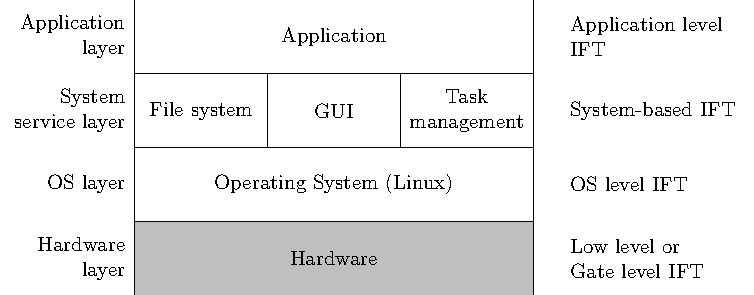
\includegraphics{c2_soa/img/system_layer.pdf}
    \caption{Simplified representation of the different layers in an embedded system}
    \label{fig:levels_system}
\end{figure}

Tracking information can be performed at various levels, from the application level to the hardware level. Each level offers distinct advantages and disadvantages.
For instance, application-level tracking might provide detailed insights and user-friendly interfaces, while hardware-level tracking offers more granular data and real-time monitoring but can be more complex and costly.
The following subsections explore these different levels, highlighting their respective benefits and limitations.


\subsubsection{Software-based DIFT}
\paragraph{Application level DIFT} tracks information flows between application variables. The programmer has to integrate data tagging inside his program and use a modified compiler or analyse his program to check if no security violation happened.
One application for DIFT at application level is language-based. Several security extensions have been proposed for existing programming languages.
JFlow~\cite{M-99-popl} is one of the first works that has described an extension of the Java language by adding statically-checked information flow annotations.

Multiple works introduce DIFT extensions for different languages, for example, such as JavaScript~\cite{CN-15-ccs, AF-09-plas}.
Austin et al.~\cite{AF-09-plas} propose a method for tracking information flow in dynamically typed languages, focusing on addressing issues with implicit paths through a dynamic check. This approach avoids the necessity for approximate static analyses while still ensuring non-interference. The method employs sparse information labelling, keeping flow labels implicit where possible and introducing explicit labels only for values crossing security domains.
Kemerlis et al.~\cite{KPJK-12-sigplan} provide a framework, \textit{libdft}, which is fast and reusable and applicable to software and hardware. \textit{libdft} provides an API for building DFT-enabled tools that work on unmodified binaries.

\paragraph{OS level and System-based DIFT} track and tag files (read or written) used by the application.
The main advantage of this approach is that it reduces the number of information flows, which lead to an improvement of the runtime overhead compared to application based DIFT.
% In the other side, the main disadvantage of this approach is that it results in more false positives than the application-level approach.

TaintDroid~\cite{EGHTCCJMS-14-tocs} introduces an extension to the Android mobile phone platform designed to monitor the flow of privacy-sensitive data through third-party applications. Operating under the assumption that downloaded third-party applications are untrusted, TaintDroid tracks in real-time how these applications access and handle users’ personal information. The primary objectives are to detect when sensitive data is transmitted out of the system by untrusted applications, and to enable phone users or external security services to analyse these applications. They store the tag adjacent to data for spatial locality. This may cause large performance and storage overheads, as the tag fetching requires extra clock cycles for memory access.
HiStar~\cite{ZBKM-11-commacm} is an OS that has been designed to provide precise data specific security policies. The authors propose to assign tags to different objects in the operating system instead of data.


\subsubsection{Software and Hardware Co-Design-Based DIFT}
This type of design combines the features of both software DIFT and hardware DIFT. Using binary instrumentations and a modified compiler, the hardware and software co-design can provide the best of these two categories of DIFT: flexible security configuration and fine-grained protection with low impact on performances~\cite{CGDJ-21-micromac, BSMCVEJCO-21-acmcsur}.

One example of this type of DIFT is RIFLE~\cite{VBCROBRVA-04-micro}, a runtime information-flow security system designed from the user's perspective, provides a practical means to enforce information-flow security policies on all programs by leveraging architectural support. RIFLE works with every programs that run on a system, and policy decisions are left to the user, not the programmer.
Townley et al.~\cite{TKPAY-19-micro} presented LATCH, a generalizable architecture for optimizing DIFT. 
LATCH exploits the observation that information flows under DIFT exhibit strong spatial and temporal locality, with typical applications manipulating sensitive data during limited phases of computation. The main objective is to detect attacks on the integrity of the system. The architecture consists of a software-assisted hardware accelerator (S-LATCH) running on a single simulated core. The software component of S-LATCH propagates tags, while the hardware accelerator monitors the data accessed by the program to detect tags. 
Porquet et al.~\cite{PS-13-codes} presented WHISK, a whole system DIFT architecture implemented within a hardware simulator. WHISK stores tags and data separately in memory locations to keep low area overhead and improve flexibility and to better accommodate the integration of hardware accelerators. The software subsystem uses the exokernel-based MutekH operating system and provides support for tag page allocation, configuration of the page table cache, and interrupt management for writing to untagged pages.

\subsubsection{Hardware-based DIFT}
Dalton et al.~\cite{DKK-07-sigarch} report that software DIFT solutions add significative runtime overhead, up to a slow-down of 37 times ! Therefore, in order to improve the execution time to be more on-the-fly, the idea is to directly implement the DIFT into the hardware, but the trade-off is flexibility.
This subsection discusses the hardware-based DIFT designs, including gate-level DIFT designs and micro-architecture-level DIFT designs. Surveys~\cite{HAK-21-acmcsur,BSMCVEJCO-21-acmcsur} present an overview on all hardware DIFT techniques. They developed a taxonomy for them and use it to classify and differentiate hardware DIFT tools and techniques.

\paragraph{Off-Core DIFT} operations are performed on a dedicated coprocessor working in parallel of the main core.
The main drawback is that this approach needs a support from the OS for the synchronisation between data computations and tags computations in order to stall one core if it needs to wait the other. But on the other hand, its advantage is that it does not require internal hardware modifications to the main core.

Kannan et al.~\cite{KDK-09-dsn} described one of the first work using a coprocessor to improve tag computation runtime overhead. Traditional hardware DIFT systems require significant modifications to the processor pipeline, which increases complexity and design time. Figure~\ref{fig:offcore_dift} represents how an off-core DIFT would be implemented. Kannan et al. uses this idea for implementing their solution.
This coprocessor handles all DIFT functionalities, synchronizing with the main processor only during system calls. This design eliminates the need for changes to the main processor's pipeline, logic, or caches, making the solution more attractive. The coprocessor is small, with an area footprint of about 8\% of a simple RISC core, and introduces less than 1\% runtime overhead for SPECint2000 applications benchmark. The paper demonstrates that the coprocessor provides the same security guarantees as in-core DIFT architectures, supporting multiple security policies and protecting various memory regions and binary types. This approach offers a balanced solution in terms of performance, cost, complexity, and practicality compared to existing DIFT implementations.

\begin{figure}[ht]
    \centering
    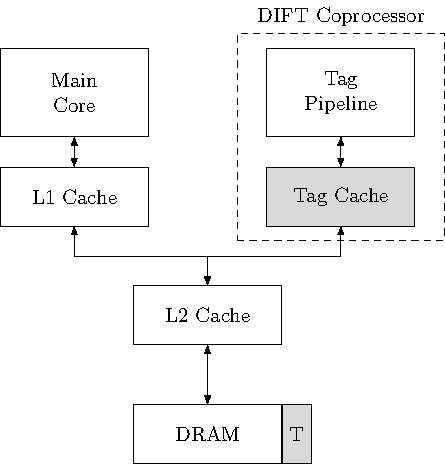
\includegraphics{c2_soa/img/offcore.pdf}
    \caption{Representation of a Hardware Off-Core DIFT (inspired by Figure 1 of~\cite{KDK-09-dsn})}
    \label{fig:offcore_dift}
\end{figure}

Wahab et al.~\cite{WCAHLG-17-fpl, WCAHBLG-18-reconfig} developed a DIFT using the ARM CoreSight debug component to extract a trace.
However, the debug component could only extract limited information about the application executing on the core. Therefore, some instrumentations have been required to recover the complete program trace. The information obtained from the trace is then sent to a dedicated DIFT coprocessor, which analyses the instruction trace and propagates tags according to a security policy. In terms of performance and area footprint, the proposed solution in~\cite{WCAHLG-17-fpl} gives around 5\% of communication overhead and an area overhead of 0.47\% from the baseline CPU, i.e. Cortex-A9 without a DIFT, and a power consumption increased by 16\%; while in~\cite{WCAHBLG-18-reconfig}, the solution gives a communication overhead of 335\%, an area increased by 0.95\% and a power consumption increased by 16.2\%.

\paragraph{Off-Loading DIFT} uses a dedicated core of a multicore CPU~\cite{CKSFGMRRRV-08-sigarch,VHYR-08-cca,RGMRCKR-08-spaa}. Figure~\ref{fig:offloading_dift} represents Off-Loading DIFT principle with a core running the application and another, in parallel, running the DIFT analysis on the application trace. The application core is instrumented in order to generate a trace and compress it. The trace includes executed instructions and packs main information such as PC address, register operands. This trace is then sent to the DIFT core via the L2 cache. Finally, the security core will decompress the trace and realise tag computation in order to check whether an illegal information flow has been done. The notion of illegal information flow is specified thanks to a DIFT security policy.
The main advantage is that hardware does not need to know DIFT tags or policies and does not need a coprocessor with the management of the synchronisation between the two processors.  But the main drawback is that it requires a multicore CPU, reducing the number of core available and increasing the power consumption due to the application trace analysis. In an embedded system where power consumption is a critical factor, this solution is difficult to consider.

\begin{figure}[ht]
    \centering
    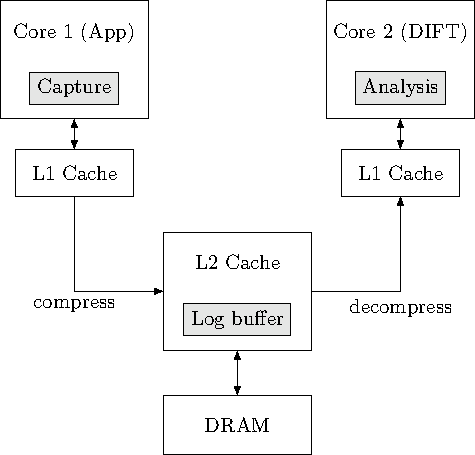
\includegraphics{c2_soa/img/offloading.pdf}
    \caption{Representation of a Hardware Off-Loading DIFT (inspired by Figure 1 of~\cite{KDK-09-dsn})}
    \label{fig:offloading_dift}
\end{figure}

\paragraph{In-Core DIFT} relies on a deeply modified processor pipeline which needs to integrate tag computations inside the main core in parallel of data computations. This approach is highly invasive, but does not require any additional cores or coprocessors to operate and introduces no overhead for intercore synchronisation. Overall, its performance impact in terms of clock cycles over native execution is minimal. On the other hand, the integrated approach requires significant modifications to the processor core. All pipeline stages must be modified to add tags, a dedicated register file, a tag computation unit, and first level of caches must be added to store tags in parallel with the regular blocks into the processor core. Processor manufacturers do not prioritise this type of approach, and as most processors are not open to the public, it is difficult to modify them. Figure~\ref{fig:incore_dift} shows the architecture of an In-Core hardware DIFT. When the processor fetches an instruction, its associated tag is sent in parallel. In the decode stage, the instruction is decoded while the security decode module decodes the security policy to determine how the tag should be propagated and checked. When the instruction is executed, the tag is sent to a tag ALU to be checked. Then, if the tag conforms to the security policy, the tag, and the ALU output are saved into the Tag Register File, or possibly, stored in memory. Otherwise, if the tag does not conform, the DIFT mechanism detects the security violation and can raise an exception. The DIFT reaction policy is not an integral part of DIFT but depends on the higher-level OS or software.

\begin{figure}[ht]
    \centering
    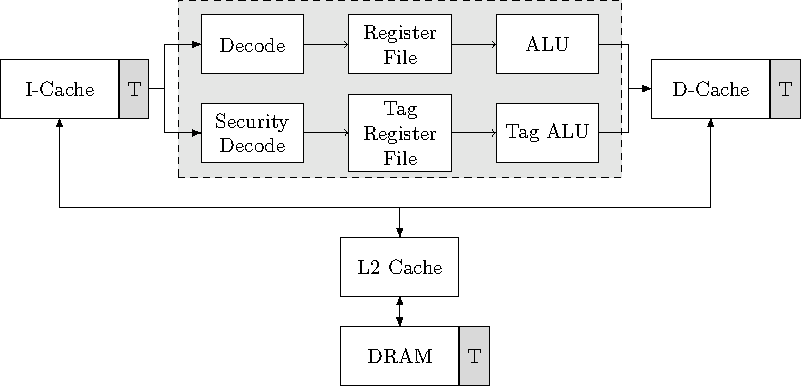
\includegraphics{c2_soa/img/incore.pdf}
    \caption{Representation of a Hardware In-Core DIFT (inspired by Figure 1 of~\cite{KDK-09-dsn})}
    \label{fig:incore_dift}
\end{figure}

Suh et al.~\cite{SLD-04-sigplan} proposed an approach in which the OS identifies a set of input channels as spurious, and the processor tracks all information flows from these inputs. Thanks to this tracking, the processor can detect various threats, such as attacks targeting instructions or jump addresses. If the security policy detects something malicious in hardware, the OS will process the exception. They use a 1-bit tag, which means only two ways of representing security levels. They present two security policies that track different sets of dependencies. Implementing the first policy incurs, on average, a memory overhead of 0.26\% and a performance decrease of 0.02\%. The second policy incurs, on average, a memory overhead of 4.48\% and a performance decrease of 0.8\%, and requires binary annotation unlike the first policy.

Dalton et al.\cite{DKK-07-sigarch} presented a DIFT architecture, Raksha, to support a flexible security configuration at runtime. They extended all storage locations including registers, caches and main memory with tags, they modified the ISA instruction to propagate and check tags. In this solution, they use 4-bit tags for each word.
The authors provided two global sets of configuration registers, i.e., Tag Propagation Registers (TPR) and Tag Check Registers (TCR), to configure the security policy at runtime. There is one pair of TPR/TCR for each of the four security policies. The configuration register could be configured only in high processor privilege (trusted) mode. Moreover, the tag propagation and check could only be disabled in trusted mode. However, the security policy is difficult to update when the architecture is deployed.
The Raksha prototype is based on the Leon SPARC V8 processor, a 32-bit open-source synthesizable core, and implemented onto an FPGA board.

Palmiero et al.~\cite{PDGLC-18-hpec} implemented a DIFT framework, D-RI5CY, on a RISC-V processor and synthesized it on a Field Programmable Gate Array (FPGA) board with a focus on IoT applications. The proposed design tags every word in data memory with a 4-bit tag and every general register with a 1-bit tag. Similarly to~\cite{DKK-07-sigarch}, Palmiero et al.~\cite{PDGLC-18-hpec} also adopted global configuration registers to customise the rule of tag propagation and checking. Each type of instruction has its own rule and can be modified separately. This method provides a more fine-grain tracking than Raksha. This solution is described in detail in Chapter~\ref{section:driscy}.

\paragraph{Gate-Level DIFT} includes gate-level netlist, and RTL designs. The goal is to protect against hardware trojans and unauthorized behaviours. To achieve that, during the creation of the circuit, additional logic is added for each gate used in the design.

GLIFT~\cite{TWMMCS-09-asplos} is a well-established IFT technique. All information flows, both explicit and implicit, are unified at the gate level. GLIFT employs a detailed initialisation and propagation policy to precisely track each bit of information flow, by adding additional logic for each gate used in the design. By analysing how inputs influence outputs, GLIFT accurately measures true information flows and substantially reduces the false positives typically associated with conservative IFT techniques.
Hu et al.~\cite{HOITSMK-11-tcad} established the theoretical foundation for GLIFT. They introduced several algorithms for generating GLIFT logic in large digital circuits. Additionally, the authors identified the primary source of precision discrepancies in GLIFT logic produced by various methods as static logic hazards or variable correlation due to reconvergent fan-outs. Many other works have been done on GLIFT to attempt a decrease of the logic complexity.

%%%%%%%%%%%%%%%%%%%%%%%%%%%%%%%%%%%%%%%%%%%%%%%%%%%%%%%%%%%%%%%%%%%%%%%%%%%%%%%%%%%%%%%%%%%%%%%
\section{Physical Attacks}
\label{section:physicalAttacks}

This section presents an overview of the state of the art on physical attacks. We introduce the different types of physical attacks and their methods to recover secret information. Firstly, we begin with Reverse Engineering, how to retrieve information from a product to recover useful information.
Secondly, we address Side-Channel Attacks (SCA), how to use information leakage to recover useful information and how to analyse them.
Finally, we introduce fault injection attacks. We define the different possibilities of injection and how to achieve them.

\subsection{Reverse Engineering}
Reverse engineering refers to the process of information retrieval from a product, ranging from aircraft to modern Integrated Circuits (IC). Reverse engineering of IC is a complex process that involves analysing and understanding the design, functionality, and operation of existing hardware. This technique is used for various purposes in the electronics industry, such as to gain a full understanding of its construction and or functionality~\cite{QCFASWCT-16-emergTech}.
To reverse engineering a chip~\cite{FSKWERP-17-ivsw}, an attacker needs to remove the chip protection in order to observe it thanks to a scanning electron microscope (SEM) or another method Focused Ion Beam (this method is explained in Chapter~\ref{subsubsection:invasiveAttacks}). Also knowing the region of interest is beneficial as the planar surface can be reduced significantly.

\subsection{Side-Channel Attacks}
Side-channel attacks exploit information leakages on the circuit behaviour such as power consumption, electromagnetic (EM) radiation or the execution time of an application.
This type of attack does not call into question the theoretical integrity of the target algorithm, but aims to recover information by devious means due to its implementation. During data processing, the switching between different states requires time and minimal energy dissipation, the variations of which can be analysed by the attacker.
This information allows the attacker to access secret data such as a password, or cryptographic key. The origin of these attacks date back to the \mbox{TEMPEST} program from NSA~\cite{F-72-nsa}. They described the vulnerabilities of a cryptographic implementation from their electromagnetic emissions, depending on the input and data.

Figure~\ref{fig:sca} represents the different methods of SCA on a microprocessor. The main idea is to have an application running on the processor and an attacker will use one method to trace the application multiple times to recover secret information (e.g. cryptographic key, password, private data, etc.).

\begin{figure}[ht]
    \centering
    \includegraphics[page=3, width=.75\textwidth]{c2_soa/img/physicalAttacks.pdf}
    \caption{Representation of the different methods of side-channel attacks}
    \label{fig:sca}
\end{figure}

Multiple possibilities exist to exploit SCA.
As seen on Figure~\ref{fig:sca}, power analysis exploits time differences in target power consumption during sensitive executions. Modern systems contain billions of transistors (up to 208 billions transistors for an Nvidia GPU GB200 Grace Blackwell\footnote{\hfill\url{https://nvidianews.nvidia.com/news/nvidia-blackwell-platform-arrives-to-power-a-new-era-of-computing}}).
These transistors act as voltage switches and as they are continually switched on/off during execution, they cause voltage variations that can be observed and measured using equipments and devices (oscilloscope, voltmeter, etc.). These data are analysed and from a certain number of data, an attacker can deduce secrets~\cite{KJJ-98-crypto,KJJR-11-jce,GP-99-ches,LKOSECG-21-sp}.

Another possibility is to analyse the execution time of a program, also known as timing attacks and first introduced by Kocher~\cite{K-96-crypto}, that takes advantage of the fact that some sensitive computational operations vary in time depending on their secret inputs~\cite{DD-05-compnet}.
A third possibility is to exploit electromagnetic (EM)~\cite{ANM-19-di,HMHSS-12-tcrypo,KSTO-17-iccad, WDL-16-ntms,HGTVJ-22-dt} emission signatures produced when conducting logic operations. Thus, EM emissions reflect the operations of the system. In 2001, Quisquater and Samyde~\cite{QS-01-scps} extended SCA with EM analysis.
Another method is to exploit the temperature~\cite{HS-14-cardis,AZRHT-21-tvlsi} values induced by the activity of the system. This method is linked to EM emissions and power analysis, as they use traces from the system's execution.
Finally, last but not least, an attacker could use acoustic analysis~\cite{BDGPS-10-usenix,GST-17-crypto,HTM-23-eurospw} to extract confidential secret from the sound emitted by the system. This technology has been around for a long time and is used in many fields, such as sonar when the system is a submarine, a warship, or a ship to distinguish one from another.

\subsection{Fault Injection Attacks}

\begin{figure}[ht]
    \centering
    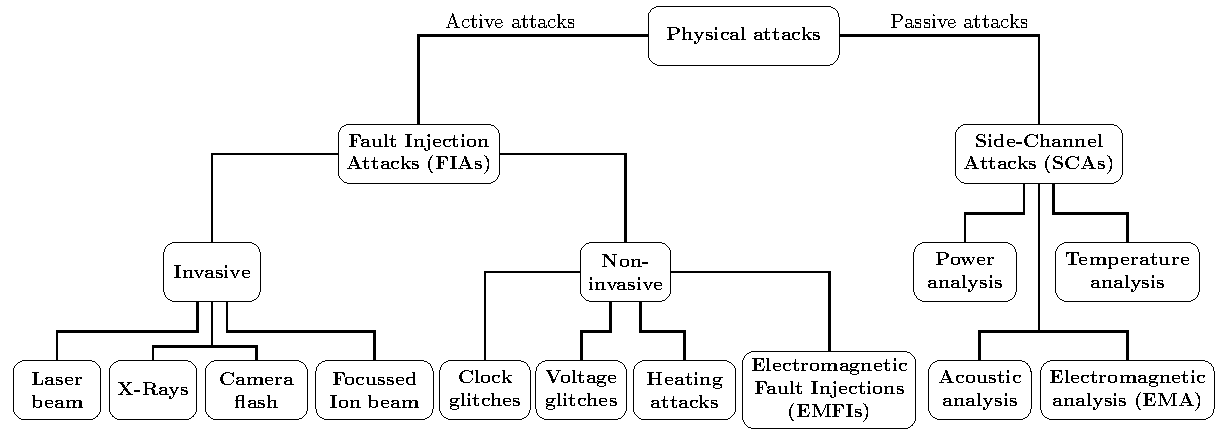
\includegraphics[width=\textwidth, page=1]{c2_soa/img/physicalAttacks.pdf}
    \caption{Taxonomy of the different methods of fault injection attacks (inspired by~\cite{CKNDCTD-21-compsec})}
    \label{fig:arbo_fia}
\end{figure}

As early as the 1970s, with advances in the space industry, anomalies in the operation of electronic circuits were observed and possibly linked to cosmic radiation outside the Earth's atmosphere~\cite{BSH-75-tns,Z-96-ibm,ZL-79-science}. These disturbances were initially found to affect the performance of electronic systems in space environments, where high-energy particles could disrupt the normal functioning of circuits. However, as transistors became smaller and required less energy to operate, similar phenomena were observed in terrestrial environments and aircraft systems. These transient disturbances, commonly referred to as "\textit{soft errors}", are now recognised as a critical issue in both space and ground electronics, affecting everything from memory chips to complex processors. Figure~\ref{fig:arbo_fia} shows a representation of a taxonomy to classify the different method of physical attacks. Each type of attacks will be explained in the following.

However, in addition to these induces cosmic faults, wanted faults exist and are known as FIAs. FIAs involves deliberately introducing a fault into the system to observe its behaviour and identify potential vulnerabilities. If the error caused by the fault does not propagate and execution of the application completes normally, the fault is ineffective. On the other hand, if the fault affects the execution of the application, causing it to fail or behave differently than expected, then the fault is effective. These faults can impact the performance, functionality, and reliability of the circuit. These attacks can induce errors in internal electronic components, which can be utilised to recover cryptographic keys and other secret data.
These attacks have been vastly studied since their first introduction by Boneh et al. in 1997~\cite{BDL-97-eurocrypt,BDL-01-crypto}. Multiple studies or surveys~\cite{ZAV-06-jarab, BCNTW-06-procieee, CKNDCTD-21-compsec, PBR-15-dtis, YSW-18-hss, BH-22-access} present the different sources of FIAs.
Figure~\ref{fig:fia} presents a summary of the different methods of FIAs, the figure does not represent all possible methods. Each of these attacks requires equipment which is more or less expensive and easy to acquire, ranging from a few hundred euros (clock glitches, voltage glitches) to several hundred thousand (Laser, X-Ray, Focused Ion Beam).

As shown in the Figure~\ref{fig:arbo_fia}, these attacks are categorised as transient or permanent, and invasive or non-invasive.
The effect of a transient fault lasts for a limited period of time. These faults rarely do any lasting damage to the component affected, although they can induce an erroneous state in the system. Their aim is to temporarily disrupt the program control flow or corrupt the results of an instruction to gain unauthorised access to sensitive code and data.
By opposition, permanent faults or destructive faults, created by purposely inflicted defects to the chip’s structure, have a permanent effect. Once inflicted, such destructions will affect the chip’s behaviour permanently and persist irrespective of device restarts and resets.

Invasive attacks involve major alteration to the Device Under Test (DUT), such as decapping the System-on-Chip (SoC) to expose its internals and remove any protective layers. These processes risk irreparable damage or destruction of the target under evaluation, potentially leading to permanent data loss.

Non-invasive attacks require no tampering of the DUT. They are able to mask their presence as they have no effect on the system other than the faults they inject.

\begin{figure}[ht]
    \centering
    \includegraphics[page=2, width=.75\textwidth]{c2_soa/img/physicalAttacks.pdf}
    \caption{Representation of the different methods of fault injection attacks}
    \label{fig:fia}
\end{figure}

\subsubsection{Invasive attacks}
\label{subsubsection:invasiveAttacks}
Invasive attacks need to decapsulate the chip or the Integrated Circuit (IC).
Decapsulating a die or an IC is a process used to expose the internal components of an IC, typically for failure analysis or reverse engineering. The goal is to carefully remove the protective encapsulation, which shields the silicon die and is typically made of epoxy or ceramic, without causing damage to the internal structures. There are several methods to achieve this, each suited to different packaging materials and levels of precision, ranging from chemical processes to advanced techniques like laser ablation and plasma etching.

The most common method is chemical decapsulation, which involves etching away the epoxy with concentrated acids such as nitric or sulphuric acid. This process requires safety precautions such as protective clothing and neutralisation of the acids after removal of the encapsulation. It is an effective but dangerous process and requires careful control to avoid damaging the die, as over-etching can cause irreversible harm.

Another method is laser decapsulation, which uses a precision laser to remove the encapsulation material layer by layer. This technique is highly accurate and reduces the risk of damage to the die, but it is expensive and requires specialised equipment. Mechanical decapsulation involves physically grinding or cutting away the encapsulation, but has a high risk of damaging the die, especially when approaching the final layers.

Plasma etching is a more advanced technique that uses ionised gases to gradually etch away the encapsulation material. It offers high precision but is slower than other methods and is typically used in research or industrial environments. Whatever method is used, safety precautions are essential, especially when dealing with hazardous chemicals and sensitive materials.

Figure~\ref{fig:decapsulating_die} shows three different steps to decapsulate a circuit. To be noted, this processor is the AMD Zen2 EPYC 7702 server processor, which is not for embedded systems.

\begin{figure}[ht]
    \centering
    \begin{subfigure}[b]{0.3\textwidth}
        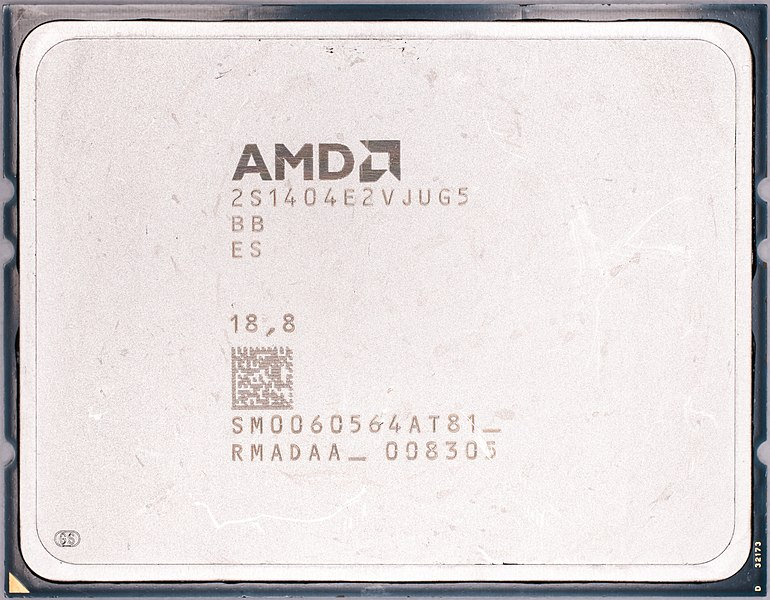
\includegraphics[width=\textwidth]{c2_soa/img/epyc_7702_initial.jpg}
        \caption{Initial die from an AMD Zen 2 EPYC 7702 server processor.}
        \label{fig:initial_die}
    \end{subfigure}
    \hfill
    \begin{subfigure}[b]{0.3\textwidth}
        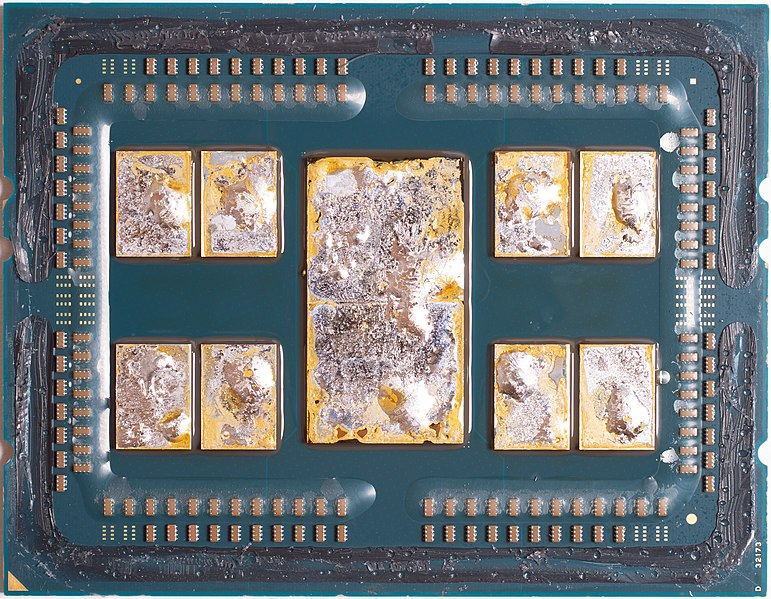
\includegraphics[width=\textwidth]{c2_soa/img/epyc_7702_delidding.jpg}
        \caption{\hfill AMD EPYC 7702 after CPU delidding.}
        \label{fig:delidding_die}
    \end{subfigure}
    \hfill
    \begin{subfigure}[b]{0.3\textwidth}
        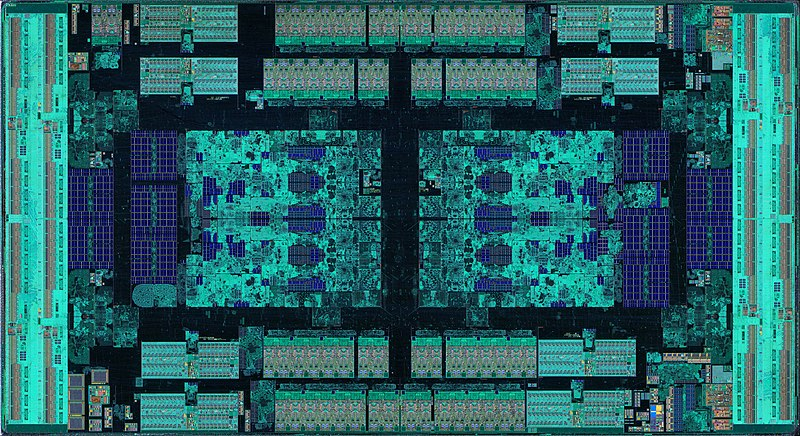
\includegraphics[width=\textwidth]{c2_soa/img/epyc_7702_packagedRemoved.jpg}
        \caption{\hfill Die shot of the centre die, after removal from processor package.}
        \label{fig:packagedRemoved_die}
    \end{subfigure}
    \caption{Three steps to decapsulate a die (from~\cite{decapping-19-wikipedia})}
    \label{fig:decapsulating_die}
\end{figure}


\paragraph{Camera flash/light source} is a type of optical attack. The attacker needs to decapsulate the chip, and the strong radiation emitted by the flash directed at the silicon surface can cause the blanking of memory cells where constant values are stored for algorithms execution (e.g., the AES S-Boxes). These attacks are inexpensive, but, on the other hand, they are not very accurate. Skorobogatov et al.~\cite{SA-02-ches} used a flashgun for \$30 while being able to change any bit of an SRAM array.

Schmidt and Hutter~\cite{SH-07-austrochip} present practical attacks on implementations of RSA that use Chinese Remainder Theorem (CRT). These attacks have been performed into a cryptographic device through optical and EM injections. They use a laser diode  as a light source, the diode emits a light  beam of \SI{100}{\milli\watt} with a wavelength of \SI{785}{\nano\metre}. The light from the diode is guided thanks to a fibre-optic of 1~mm in diameter.
Guillen et al.~\cite{GGD-17-cosade} present a low-cost fault injection setup, around a couple of hundred euros, which is capable of producing localized faults in modern 8-bit and 32-bit microcontrollers. This setup does not require handling dangerous substances or wearing protection equipment. The fault produced by this setup are able to successfully attack real-world cryptographic implementations, such as the NSA’s Speck lightweight block cipher~\cite{RDJSBL-13-nsa}.

\paragraph{Laser beam} is another type of optical attacks.
The injected fault is similar to the one used with a camera flash, except that it is a lot more precise and is capable of always inducing faults.
The main downside of this method is that it requires a high expertise.
Dutertre et al.~\cite{DBCDFFGHLMDPR-18-fdtc} explain the theory behind this technique at the lowest level.

\begin{figure}[ht]
    \centering
    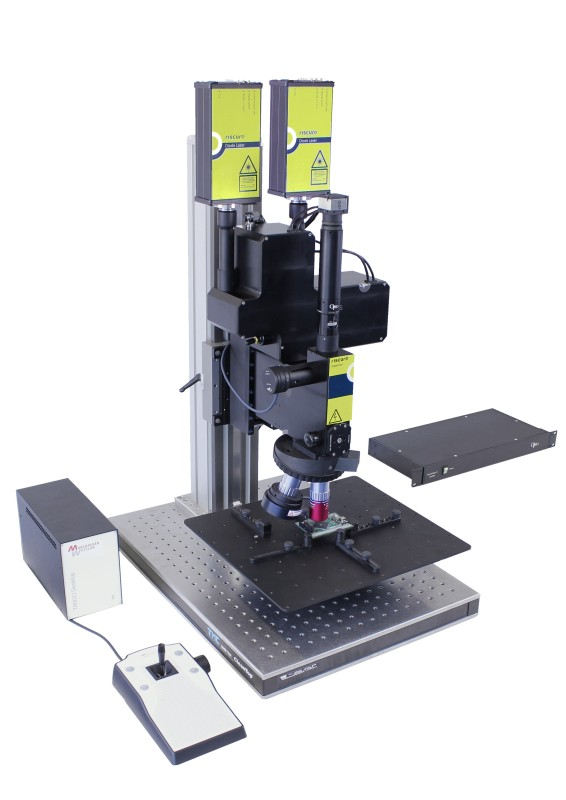
\includegraphics[width=0.5\textwidth]{c2_soa/img/LS2.jpeg}
    \caption{Example of a laser fault injection station (by Riscure Laser Station 2~\cite{riscure_station})}
    \label{fig:ls2}
\end{figure}

Figure~\ref{fig:ls2} shows an example of a laser fault injection station made by Riscure.
It contains powerful red and NIR diode lasers (respectively \SI{14}{\watt}, and \SI{20}{\watt}). The red laser is designed for frontside testing of smart card chips, and in combination with the optics it produces a spot size of 6 * \SI{1.4}{\micro\metre} on the chip surface. The near-infrared laser is designed for backside testing of smart card chips. This powerful diode laser penetrates the chip substrate to reach the transistors.
This station automates the surface scanning process, offers precise control of laser power, and injects pulses with a small spot size. It has a precise and fast response thanks to a trigger and the ability to perform multi-glitching.

Using a laser beam, a single bit~\cite{CMDMRD-19-host} in a memory can be set (from logical 0 to logical 1) or reset (from logical 1 to logical 0) by attacking either the frontside or the backside of the chip.
Today, the capabilities of laser injection mechanisms make it possible to carry out attacks with multiple faults.
Colombier et al.~\cite{CGVCBLC-22-cardis} use a four-spot laser bench to inject up to 4 non-contiguous bits in a single cycle, or multiple non-contiguous bits over multiple cycles. This fault injection mechanism therefore makes it possible to construct much more complex attacks, potentially capable of bypassing many countermeasures.

Breier et al.~\cite{JHJBC-17-hss} studied the fault mechanism of circuit logic elements in FPGA environment, and performed a practical laser fault injection into a single bit CED-protected block cipher in Xilinx Virtex-5 FPGA.
Figure~\ref{fig:lfi_setup} shows their setup to inject fault.
The chip is preprocessed by a mechanical solution in order to reduce the substrate thickness to approximatively \SI{100}{\micro\metre}. Thinner substrate leads to easier laser penetration, at the risk of destroying logic resources or routing channels on the chip.
The laser used is a \SI{20}{\watt} diode pulse laser with 5 times magnification lens, which reduce the effective maximum power to \SI{10}{\watt}. The wavelength is \SI{1064}{\nano\metre} and the spot size of the laser beam is approximatively \SI{840}{\micro\metre}$^2$.

\begin{figure}[ht]
    \centering
    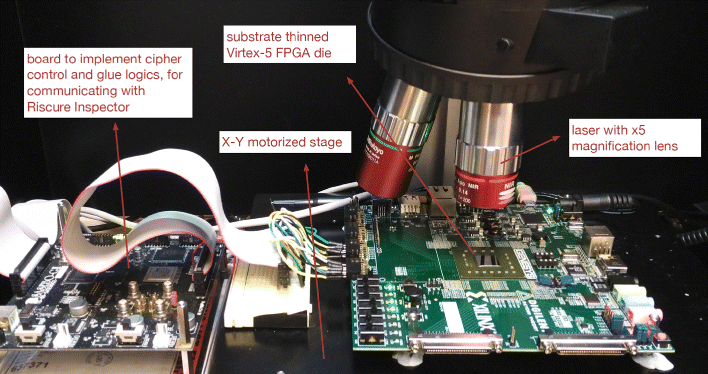
\includegraphics[width=\textwidth]{c2_soa/img/lfi_setup.png}
    \caption{Example of a laser fault injection setup (by~\cite{JHJBC-17-hss})}
    \label{fig:lfi_setup}
\end{figure}

\paragraph{Focused ion beam} is the most accurate and powerful fault injection technique. Focused ion beam (FIB) enables an attacker to arbitrarily modify the structure of a circuit, reconstruct missing buses, cut existing wires and rebuild them. FIB systems typically use liquid metal ion sources, where their low atomic mass and the relatively low energy of these ions make them suitable for high-resolution imaging and precision milling of materials at the nanoscale~\cite{FVMBMWP-23-wfiot}.

FIB can operate at a precision of \SI{2.5}{\nano\metre}, which is the size of a transistor in an actual IC.
FIB workstations require very expensive consumables and a strong technical background to fully exploit their capabilities. The only limit to the FIB technology is the diameter of the atoms whose ions are used as a scalpel. Currently, the most common choice is Gallium, which sets the lower bound to roughly \SI{0.135}{\nano\metre}.

These attacks are out of the scope for classical considered attackers due to the cost of the equipment. However, these attacks can be considered for critical systems such as military equipment. The granularity of the faults that can be introduced with FIB makes it possible to emulate both physical defects (such as stuck-at faults) and more complex logical faults.

Figure~\ref{fig:fib_setup} shows the principle of how FIB works. The gallium ($Ga^+$) primary ion beam hits the sample surface and sputters a small amount of material, which leaves the surface as either secondary ions ($i^+$ or $i^-$) or neutral atoms ($n^0$). The primary beam also produces secondary electrons ($e^-$). As the primary beam strikes on the sample surface, the signal from the sputtered ions or secondary electrons is collected to form an image.

Torrance and James~\cite{TJ-09-ches} report a successful reconstruction of an entire read bus of a memory containing a cryptographic key without damaging the contents of the memory.

\begin{figure}[ht]
    \centering
    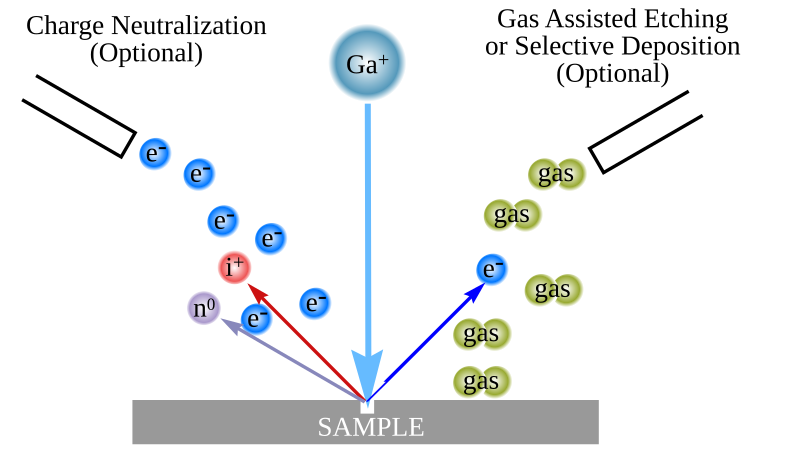
\includegraphics[width=0.5\textwidth]{c2_soa/img/fib.png}
    \caption{The principle of FIB (by~\cite{fib-24-wikipedia})}
    \label{fig:fib_setup}
\end{figure}

\subsubsection{Non-invasive attacks}
Non-invasive attacks involve inducing errors in a system without physically tampering with the device. These attacks exploit external influences like electromagnetic interference, voltage glitches, or clock signal manipulation to cause faults during the device's operation. Unlike invasive methods, which require dismantling or altering the hardware, non-invasive techniques leave no physical traces, making them harder to detect. By injecting faults at precise moments, attackers can bypass security mechanisms, retrieve sensitive data, or alter the device's intended functionality.

\paragraph{X-Rays} is another approach to inject fault very precisely, but this method is not invasive as \mbox{X-Rays} can go through the IC package without the need of decapsulating it. Another advantage is that X-Ray have a lot smaller wavelength, down to \SI{0.01}{\nano\meter}, than laser injection which are limited to the wavelength of their light source, down to \SI{1}{\micro\meter}.
The injected fault is semi-permanent, and to make it disappear, the attacker has to heat up the device. This differs from other techniques, where the fault can disappear a few cycles after injection.
This technique can be compared as a non-invasive FIB techniques. X-ray provides many opportunities for attacking electronic circuits. Among them, we can note the possibility to cause permanent faults in cryptographic algorithms, deactivation of countermeasures, reprogramming of memories, etc.

Anceau et al.~\cite{ABCMRT-17-ches, BAMCST-23-dft} propose an approach for modifying the behaviour of a transistor in the memory of a circuit using focused X-ray beams. 
They use the European Synchrotron Radiation Facility (ESRF), in Grenoble, France.
Grandamme et al.~\cite{GBD-23-paine} show efficiency of X-Ray faults injection on flash and EEPROM memories for powered off devices. They also describe a fault model according to their experimental results and propose a solution to correct a part of the fault.

\paragraph{Clock glitches} are a type of fault injection attack that targets the timing of a system's clock signal to introduce errors into its operation. It is primarily used to disrupt the normal execution of a digital circuit, such as a microcontroller or a cryptographic processor, by momentarily altering its clock frequency.

In this attack, the adversary deliberately introduces short pulses or glitches into the clock signal. These glitches can cause the system to either skip instructions, execute them incorrectly, or process data in unintended ways. By carefully timing these glitches, the attacker may manipulate sensitive operations, such as cryptographic computations, potentially exposing vulnerabilities like secret keys, bypassing security checks, or triggering unintended behaviour in the device.

\begin{figure}[ht]
    \centering
    \includegraphics[page=5]{c2_soa/img/physicalAttacks.pdf}
    \caption{Representation of the parameters of a clock glitch attack}
    \label{fig:clock_glitch_parameters}
\end{figure}

Figure~\ref{fig:clock_glitch_parameters} represents the three parameters that are taking into account for this kind of attacks:
\begin{itemize}
    \item Delay: the time between the rising edge of the trigger signal and the rising edge of the targeted device's clock cycle.
    \item Offset: determines when the glitch is applied relative to the system's clock cycle.
    \item Width: the duration of the glitch.
\end{itemize}

The duration of both offset and width can not be too large or too short. Because too short values will lead to too short range to obtain a timing violation, and too large values will not modify the instruction behaviour but can overcome the critical path.

Figure~\ref{fig:clock_glitch} represents an example of a clock glitch attack, where you can see the \textit{Normal Clock} is not faulted, and its behaviour is very regular. While, the \textit{Glitched Clock} suffers from a glitch where an abnormal cycle is introduced, and it induces an additional instruction execution. Under real conditions, the injected clock cycle would not last long enough for the instructions to execute normally. Hence, in these conditions, an instruction skip would happen.

\begin{figure}[ht]
    \centering
    \includegraphics[page=4]{c2_soa/img/physicalAttacks.pdf}
    \caption{Representation of a clock glitch attack (inspired by~\cite{newae_clock})}
    \label{fig:clock_glitch}
\end{figure}

Balasch et al.~\cite{BGV-11-fdtc} show clock glitches can cause an instruction skip during the execution of a program.

\paragraph{Voltage glitches} exploit the power supply of a digital system to introduce errors in its operation. Instead of manipulating the clock signal, this technique involves deliberately varying the voltage supplied to the system, typically by creating sharp, transient drops or spikes in the power supply (i.e. under- or overvolting)~\cite{BBPP-09-fdtc}, or redirecting it to ground to generate voltage drops, known as "glitches" in order to generate faults of one or multiple bits. This can corrupt the contents of memory units or force microprocessors to misinterpret or even skip program instructions.
Such as clock glitches, voltage glitches can be used to bypass authentication mechanisms, extract cryptographic keys, or cause logic errors that undermine the security of a device. It's a widely recognised threat in hardware security, especially in applications where physical access to devices is possible, such as smart cards, IoT devices, and hardware security modules.

\begin{figure}[ht]
    \centering
    \includegraphics[page=6, scale=1.25]{c2_soa/img/physicalAttacks.pdf}
    \caption{Representation of a voltage glitch attack}
    \label{fig:voltage_glitch}
\end{figure}

Figure~\ref{fig:voltage_glitch} represents the three parameters that are taking into account for this kind of attacks:
\begin{itemize}
    \item Delay: the time between the rising edge of a trigger signal and the injection.
    \item Amplitude: the voltage value of the injection or the drop introduced. In Figure~\ref{fig:voltage_glitch} a drop in the voltage is represented, but the spike could be in the positive axis and then introduce an overvoltage in the circuit.
    \item Length: the time duration of the applied power variation.
\end{itemize}

Timmers and Mune~\cite{TM-17-fdtc} demonstrated voltage FIAs for Linux-based privilege escalation on an undisclosed ARM Cortex-A9-based SoC. The authors targeted the open syscall when an unprivileged application attempted to access physical memory. The application was instrumented to trigger the fault during the kernel’s access control check, which caused it to be skipped.
Timmers et al.~\cite{TSW-16-fdtc} show the use of glitch injections on the power supply to change the CPU PC register to a predetermined address while executing random kernel syscalls, generating system crashes.

\paragraph{Heating attacks} involve deliberately raising the temperature of a digital system or its components to induce malfunctions and errors. This type of attack exploits the fact that many electronic devices and integrated circuits are sensitive to temperature variations and may not operate reliably when subjected to abnormal thermal conditions.

On the other hand, these attacks have limitations in terms of both temporal and spatial precision. In other words, heating or cooling a device takes a long time due to thermal inertia compared to the speed of the device's calculation and hence precise attack can not be executed.

Anagnostopoulos et al.~\cite{AARSGK-18-dsd} present a study of data remanence effects on SRAM memories devices for temperature ranging between \SI{-110}{\degreeCelsius} and \SI{-40}{\degreeCelsius}. From their results, they assess potential countermeasures against a new attack defined from data remanence.

Hutter et al.~\cite{HS-14-cardis} heat up a microcontroller beyond operating temperature and manage to attack an RSA software implementation.

\paragraph{Electromagnetic fault injections (EMFI)} disrupt the normal operation of a system. In this attack, an attacker generates short bursts of strong electromagnetic fields aimed at a specific part of the device, such as a microcontroller or a processor, in order to induce faults in its execution.

The goal of EMFI is to cause unintended behaviour in the target system by disturbing its internal electrical circuits. These disruptions can lead to various faults, such as skipping instructions, corrupting data, triggering incorrect logic states, or bypassing security checks. By carefully controlling the timing, location, and intensity of the EM pulses, the attacker can influence critical operations within the device, potentially gaining access to sensitive information or compromising the system's security.
EMFI is particularly effective because it does not require direct physical contact with the system. The state-of-the-art EMFI setups provide millimetre-level precision in spatial location and nanosecond-level precision in the temporal location of the EM pulse.
It's worth noting that EMFI can also be considered invasive. Some classify EMFI into a third category, known as semi-invasive attacks, because the package can be removed to allow direct access to the IC, improving EMFI efficiency and accuracy.

\begin{figure}[ht]
    \centering
    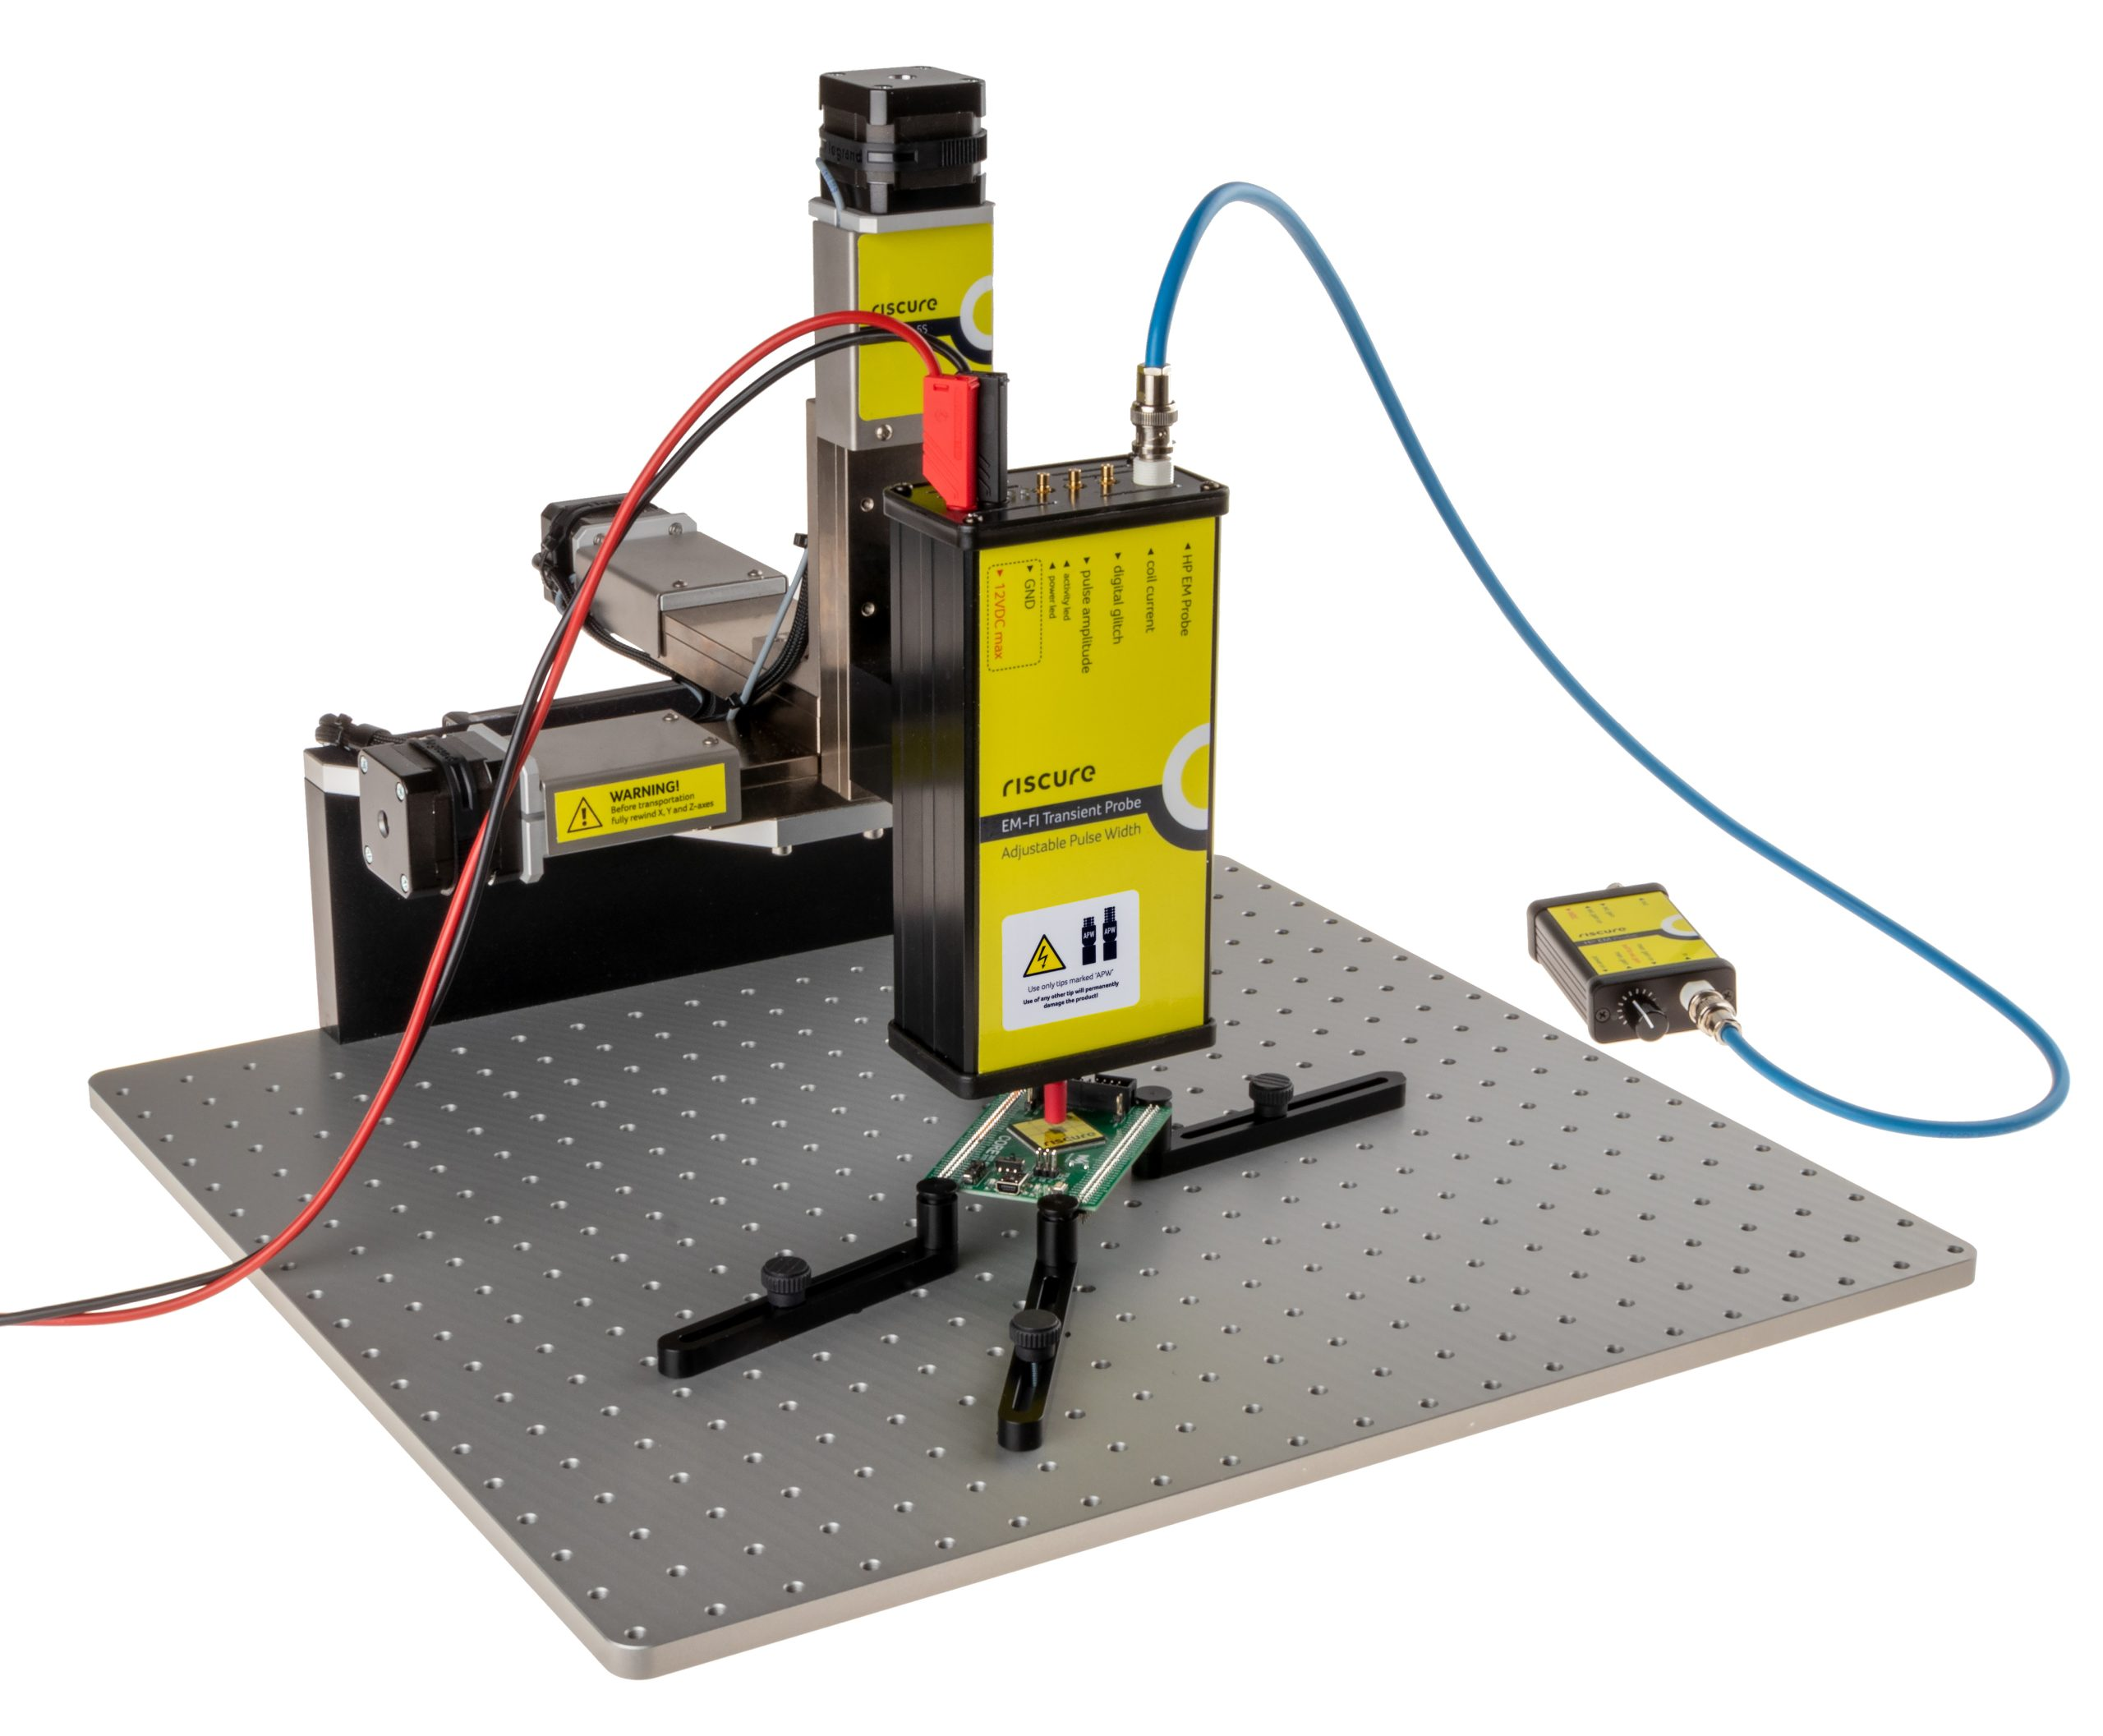
\includegraphics[width=.5\textwidth]{c2_soa/img/emfi_riscure_setup.jpg}
    \caption{Example of an EMFI attack setup (by~\cite{riscure_emfi})}
    \label{fig:emfi_setup}
\end{figure}

Dehbaoui et al.~\cite{DMMDT-13-cosade} succeeded in recovering the encryption key of an AES software implementation by injecting a short EM pulse on a 32-bit microcontroller.
Schmidt et al.~\cite{SH-07-austrochip} use a simple gas lighter to induce EM pulses onto an 8-bit microcontroller with low spatial and temporal precision.
Trouchkine et al.~\cite{TBELB-21-jce} present an approach to recover an AES key, using EMFI, by targeting the cache hierarchy and the MMU.

\subsubsection{Fault Injection techniques summary}
Table~\ref{table:fia_techniques} shows a summary of all presented techniques to realise a fault injection attack. Depending on the budget available for the attacker, and the required need for spatial and timing accuracy, the technique can be different.

Clock glitches, voltage glitches, heating attacks and camera flash can cost from few tens of Euros / US Dollars (USD) to less than \$3,000. For EMFI attacks, Chip Shouter~\cite{chipshouter} costs around \$3,000 and more precise setup can cost \$30,000~\cite{BH-22-access}. These techniques are accurate and require a low to moderate expertise on the equipment and techniques. The level of expertise required depends on both the equipment and the accuracy of the attack. The more precise the equipment, the higher the level of expertise is needed. On the other hand, for even more precise techniques, such as laser, FIB, or even X-Ray, the cost can go up to millions of USD/Euros as the equipment can be a lot more expensive, such as the equipment needed for X-Ray injection, but an attacker can recover a lot of secret data thanks to these attacks.

\begin{table}[ht]
    \centering
    \caption{Fault Injection methods summary}
    \label{table:fia_techniques}
    \begin{tabular}{@{}rccccc@{}}
        \toprule
        \textbf{Technique} & \begin{tabular}{c}\textbf{Precision}\\{\small\textbf{(time)}}\end{tabular} & \begin{tabular}{c}\textbf{Space}\\\textbf{accuracy} \end{tabular} & \textbf{Cost} & \textbf{Expertise} & \begin{tabular}{c}\textbf{Damage}\\\textbf{risk} \end{tabular} \\ \midrule
        Clock Glitches     & High                                                                                             & Low                                                               & Low           & Low                & Very low                                                       \\
        Voltage Glitches   & Moderate                                                                                         & Low                                                               & Low           & Low                & Very low                                                       \\
        Heating attacks    & Very low                                                                                         & Very low                                                          & Low           & Very low           & Moderate                                                       \\
        Camera flash       & Moderate                                                                                         & Low                                                               & Moderate      & Moderate           & High                                                           \\
        EMFI                & High                                                                                             & High                                                              & Moderate      & Low/Moderate       & Low                                                            \\
        Laser              & Very high                                                                                        & Very high                                                         & High          & High               & Very high                                                      \\
        Focused Ion Beam   & Very high                                                                                        & Very high                                                         & Very high     & Very high          & Very high                                                      \\
        X-Ray              & Very high                                                                                        & Very high                                                         & Highest       & Very high          & Very low                                                       \\
        \bottomrule
    \end{tabular}
\end{table}

\subsubsection{Fault models}
\label{section:soa_fm}
In the context of physical attacks, a fault model is a conceptual representation of how faults can occur and the effects they can have on the operation of a system. In simple terms, it describes the various ways in which a system can be altered when subjected to external perturbations.
We present the most popular fault models, which are used in the literature.

Multiple studies~\cite{BH-22-access,GMA-22-electronics,KSV-13-tvlsi,ZAV-06-jarab,YSW-18-hss} present a small overview on different fault models for fault injection attacks. Different possibilities exist depending on the equipment and the effect targeted. Otto~\cite{O-05-phd} presented a deep study and definitions of fault models.

With a low-cost equipment, an attacker can achieve instruction skip, random byte attacks, execution faults. While with higher cost equipment, this attacker is able to create bit-flip into the architecture, bit set/reset, or stuck-at-fault, temporal bit-flip, or spatial bit-flip.

Bit-flip~\cite{CMDMRD-19-host} is the modification of a bit to the logical opposite ($0 \Rightarrow 1$ or $1 \Rightarrow 0$).
Multiple bit-flips~\cite{CGVCBLC-22-cardis} are also in this category, as long as all the target bits are selected by the attacker.
There is also, spatial bit-flips change the value of two bits in one or two registers at the same clock cycle.
And finally, temporal bit-flips that change the value of two bits in one or two registers at two clock cycles.
Bit set/reset~\cite{BS-03-financialcrypto} is the modification of the bit value either to logical \texttt{1} (set) or logical \texttt{0} (reset). Again, this bit can be precisely targeted by the attacker.
Random byte~\cite{LFZD-16-fdtc} is less accurate than the previous ones as the attacker targets a byte and sets it to another random value (for example, in binary, from \texttt{0b01010101} to \texttt{0b00111001}).
Instruction skip~\cite{MDPRD-20-dtis} ignores the execution of the current processed instruction.
Stuck-at faults~\cite{MABGHMRSYV-18-fdtc} permanently set the targeted data to another value.


%%%%%%%%%%%%%%%%%%%%%%%%%%%%%%%%%%%%%%%%%%%%%%%%%%%%%%%%%%%%%%%%%%%%%%%%%%%%%%%%%%%%%%%%%%%%%%%
\section{Countermeasures against FIAs}
\label{section:countermeasuresAgainstFIA}
In the previous section, we showed the need to protect against fault injection attacks.
In this section, we will only present the countermeasures to protect a system against fault injection attacks.
Countermeasures can be implemented in software, in hardware, or even in the physical layer~\cite{BCNTW-06-procieee}.

The objectives when implementing countermeasures are:
\begin{itemize}
    \item to detect faults and react in accordance with a security policy (for example, tolerate them or attempt to correct them);
    \item to ensure that incorrect results are not usable by the attacker. 
\end{itemize}

\subsection{Countermeasures in the physical layer}
Countermeasures can be implemented in the physical layer, such as sensors that detect a perturbation. He et al.~\cite{HBB-16-space} propose a full-digital detection logic against laser fault injection. El-Baze et al.~\cite{ERM-16-date} present and validate a new sensor allowing to detect EMFI. Muttaki et al.~\cite{MZTF-22-host} introduce a universal Fault-to-Time Converter sensor that can effectively detect FIAs (clock glitch, voltage glitch, laser, EMFI) while requiring minimal overhead.

\subsection{Software countermeasures}
Software countermeasures target vulnerable parts of the code (loops, memory access, etc.). They are often relatively easy to implement compared with hardware countermeasures. However, they are more likely to be bypassed, as their implementation does not take into account the system's microarchitecture.
In addition, the cost regarding the performance of the system is significant in terms of memory requirements and execution time~\cite{BCNTW-06-procieee}. The principle of duplication, for example, doubles both the memory space required and the execution time for the protected sections.
A classic technique is to use temporal or spatial redundancy. Barenghi et al.~\cite{BBKPR-10-wess} suggest tripling instructions by storing the results in different registers. If these registers are different, it means a fault occurred.
Theißing et al.~\cite{TMSSS-13-date} implemented and systematically analysed a comprehensive set of 19 different software countermeasure strategies for protection effectiveness, time, and memory efficiency.
Chamelot et al.~\cite{CCH-22-date} present SCI-FI, a countermeasure for Control Signal, Code, and Control-Flow Integrity against Fault Injection attacks.
Laurent et al.~\cite{LBDPP-19-microproc} analyse some existing countermeasures and show how they handle precise faults extracted from the processor.
Some countermeasures propose solutions to protect the data linked to the control flow. For example, Schilling et al.~\cite{SWM-18-date} propose protecting the calculation of conditional branches while preserving the error-detection capabilities at every stage of a conditional branch. They demonstrate this by implementing an encoded comparison using AN-codes. They also integrated this countermeasure in the LLVM compiler to automatically protect conditional branches.

However, even if those countermeasures are good against FIAs, they are still sensitive against some attacks and can be bypassed by analysing the processor microarchitecture. Laurent et al.~\cite{LBDP-19-date} present an attack where they target hidden registers into a \mbox{RISC-V} processor. They show that even if a code is protected against FIAs, they can find some vulnerabilities and bypass the software countermeasures. It is then better to directly implement hardware countermeasures at the lower level to have the best protection available.

\subsection{Hardware countermeasures}
Hardware countermeasures~\cite{BCNTW-06-procieee, PTAJC-22-appSci} consist of adding hardware mechanisms to the system architecture, which makes them more effective. Adding a countermeasure introduces a loss of performance into the target system. Its implementation usually involves increasing the size of the hardware's area, reducing the maximum frequency, or increasing the power consumption. However, once the implementation is done, an evaluation of the protection is usually done to compare it and give some indications in terms of area, performance, or efficiency.
In the state of the art, multiple solutions exist to protect a system against FIAs such as information redundancy, spatial or hardware redundancy, temporal redundancy, and obfuscation.

\subsubsection{Hardware redundancy}
Hardware redundancy~\cite{JMR-07-iet, DFR-07-dsn, NDFR-08-ets} countermeasure consists of duplicating the protected circuit or part of it to compare the result obtained after computation to check if there is a difference. Figure~\ref{fig:spatial_redundancy} represents the spatial redundancy. An input is sent to two or more modules (i.e. computation blocks) and the output results will be compared, to check if an error occurred.
This type of countermeasure is the most direct and simplest, but at the same time, it is the one with the highest resource cost.
One of the most common techniques used to implement hardware redundancy is Triple Modular Redundancy (TMR). TMR involves tripling the logic and using voters to correct the error based on the majority. This means that in order to produce the correct output, two out of three signals must function correctly. However, there are large penalties in terms of area and power consumption with this method.

\begin{figure}[ht]
    \centering
    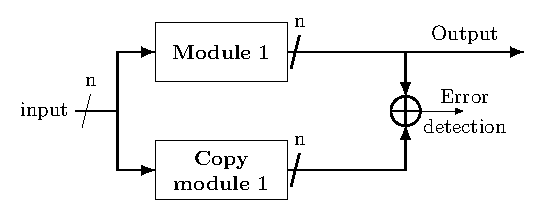
\includegraphics[page=1]{c2_soa/img/redundancy.pdf}
    \caption{Representation of hardware spatial redundancy}
    \label{fig:spatial_redundancy}
\end{figure}

\subsubsection{Temporal redundancy}
Temporal redundancy~\cite{RBMK-10-host, MVL-07-fdtc, GK-13-tcad}  is based on repeating operations in reverse. In this way, it is possible to check the result of an operation with its previous value. It significantly increases the time required. This is because it takes twice as long to perform reverse verification operations. Furthermore, protection can be achieved with more or less resources, depending on security and redundancy levels. Figure~\ref{fig:temporal_redundancy} shows how the input is saved into a register, the value is then sent to a calculation module for output and reversed in a reverse computation module to compare the value from the saved valued in the register. If the register's value differs from the value computed by the reverse module, it means that an error occurred, and then an error signal is emitted.

\begin{figure}[ht]
    \centering
    \includegraphics[page=2]{c2_soa/img/redundancy.pdf}
    \caption{Representation of hardware temporal redundancy}
    \label{fig:temporal_redundancy}
\end{figure}

\subsubsection{Instruction replay}
Another type of redundancy is to execute multiple times the same instruction or block of instructions. This redundancy, called instruction replay or instruction duplication/triplication, can be executed on one or more instructions and can be decided in software or in hardware. This solution has many advantages in terms of efficiency, but it induces large overhead in terms of performance, and area.
Manssour et al.~\cite{NLGT-22-ddecs} present a solution to avoid large performance overhead by using dedicated instructions on a RISC-V processor. While using a very small processor, 2 stages, they have a 30\% increase of area and 10\% of frequency decrease. The hardware replay allows reducing the execution time and code size compared to a full software protection (for execution time, from a factor of 3 to a factor or 2, and, for code size, from a factor of 2 to a factor or 1.3).

\subsubsection{Information redundancy}
Another approach of security is the redundancy of the information. This means that additional information is added to the data to enable error detection or correction. The most important techniques in this area are Error Detection Codes (EDC) and Error Correcting Codes (ECC).

EDC~\cite{APHBML-16-date,MKBM-14-sta,BBKMP-03-toc} is a class of countermeasures that computes the parity (odd or even) of the protected target (e.g. registers). EDC, such as parity bits, checksums, or cyclic redundancy checks (CRC), can detect these manipulations by checking the integrity of the data or computations against redundant bits or codes. The main advantage of these countermeasures is that they inevitably detect single-bit faults with a very small overhead, unlike other previous methods. This method can only detect an error, but is unable of correcting it. This method will be further developed in Chapter~\ref{chapter:simpleparity} with an implementation of a simple parity code.

Error Correcting Code (ECC)~\cite{PTCVAJ-20-iscas,DGMMNM-20-arcs,CB-06-toc}, or sometimes referred to as Error Detection And Correction Code (EDAC), ensures that even if faults are injected, the system can recover the original data or identify the presence of an error by encoding the original data with additional bits (e.g. redundancy bits). This makes ECC a robust defence mechanism against fault injection attacks, improving both data integrity and system reliability. ECC can be divided into two main families and a hybrid family: Linear Block Codes, Convolutional Codes and the hybrid Turbo or Concatenated codes. Some examples of such codes are Hamming Codes, Single Error Correction Double Error Detection (SECDED), Reed-Solomon, Low-Density Parity-Check (LDPC), BCH code, and Cyclic Redundancy Check (CRC). CRC can be considered as EDC as well as ECC. This method will be developed in Chapter~\ref{chapter:hammingcode} with the implementation and a detailed presentation of Hamming Code.

\subsubsection{Obfuscation}
Obfuscation is a technique that includes the addition of dummy cycles, during which the processor performs operations that are irrelevant to the current calculation. Another strategy is to shuffle the data to make it more difficult for the attacker to determine where to inject faults. Their effectiveness depends on their random nature. If the obfuscation is based on a constant, the attacker will only have to identify this constant to bypass the protection. On the other hand, if the obfuscation is random, the attacker will have to repeat the identification process for each new attack.

%%%%%%%%%%%%%%%%%%%%%%%%%%%%%%%%%%%%%%%%%%%%%%%%%%%%%%%%%%%%%%%%%%%%%%%%%%%%%%%%%%%%%%%%%%%%%%%
\section{Summary}
This chapter has provided an overview of the three main areas of my PhD thesis work: information flow tracking, physical attacks and countermeasures against fault injection.

The security mechanism, DIFT, is used to protect a system against software attacks such as buffer overflow, SQL injection and malware. In the remainder of this work, we are using a DIFT mechanism integrated into the hardware processor (hardware in-core DIFT) on a RISC-V processor, enabling access to the core's HDL code.

The physical attacks are diverse, ranging from the analysis of the sounds of a system or the analysis of its power consumption to fault injection using a laser or even X-rays. Their study is constantly evolving, enabling vulnerabilities in today's embedded systems to be identified with increasingly limited resources. This increases the number of potential attackers, making it all the more necessary to incorporate the concept of integrated security at the design stage, with the addition of robust countermeasures.

Finally, we provide an overview of the various existing software, hardware, and physical countermeasures against fault injection attacks. These countermeasures must be integrated within certain constraints, such as effectiveness, area overhead or performance decrease.

%%%%%%%%%%%%%%%%%%%%%%%%%%%%%%%%%%%%%%%%%%%%%%%%%%%%%%%%%%%%%%%%%%%%%%%%%%%%%%%%%%%%%%%%%%%%%%%